\begin{savequote}[45mm]
\ascii{I'm not a great programmer; I'm just a good programmer with great habits.}
\qauthor{\ascii{- Kent Beck}}
\end{savequote}

\chapter{类设计}
\label{ch:class-design}

%%%%%%%%%%%%%%%%%%%%%%%%%%%%%%%%%%%%%%%%%%%%%%%%%%%%%%%%%%%%%%%%%%%%%%%%%%%%%%%%
\section{构造与析构}

\begin{content}

\begin{regulation}
抵制设计和实现上帝类
\end{regulation}

上帝类是一种典型的代码坏味道,它与\ascii{SRP(Single Reponsibility Principle)}相违背。程序员几乎都会碰到这样的巨类,搜索其成员变量的修改点是一件痛苦的事情;成员变量在\ascii{20-30}个成员函数中穿梭,变得像全局变量一样难理解。不仅如此,修改这个巨类,代码冲突常常发生,修改这样的高度耦合的类需要高超的技能。

消除这样的巨类,关键是识别出类中的主要职责,按照\ascii{SRP}原则来分解巨类,在此不深入探讨此方面的内容\footnote{详细内容可参考\ascii{Michael C. Feathers}所著的\ascii{《Working Effectively with Legacy Code》}, 中文版名为《修改代码的艺术》}。

\begin{regulation}
明确\cpp{}的初始化规则
\end{regulation}

初始化永远是程序员心中的痛,尤其面对复杂的\cpp{}语言时。\cpp{}使用构造函数完成初始化,而构造函数使用初始化列表完成初始化的。初始化列表首先调用父类的构造函数;然后按照类中定义的的成员变量的顺序依次进行初始化。

没有显式地调用父类构造函数,编译器则自动调用父类的默认构造函数;如果对应的父类或成员变量没有默认构造函数,则需显式地调用调用特定的带参构造函数,否则编译失败。如果没有显式地调用本类的成员变量,规则也类似。

特殊地,const数据成员,引用数据成员必须在初始化列表中进行初始化。

\begin{regulation}
手工初始化内置数据类型的成员变量,\cpp{}语言并没有保证其初始化。
\end{regulation}

基本数据类型包括整形,浮点型,指针,引用等类型;当设计一个含有基本数据类型的成员变量时,必须定义构造函数完成其初始化。

TransData必须实现其对基本数据类型的成员变量的初始化,否则它们就是未定义的,其行为未定义。

\begin{leftbar}
\begin{c++}
template<typename T>
struct TransData
{
   TransData();
   ~TransData();

   void confirm()
   void revert()

private:
   T values[2];
   unsigned char valid :1;
   unsigned char memoed :1;
   unsigned char unstable :1;
   unsigned char currentIndex :1;
   unsigned char :4;
};

template<typename T>
TransData<T>::TransData() : valid(0), memoed(0), unstable(0), currentIndex(0)
{
}
\end{c++}
\end{leftbar}

\begin{regulation}
在初始化列表中实现对非内置数据类型的初始化
\end{regulation}

非内置数据类型指类类型,如果它们没有在初始化列表中初始化,则编译器默认调用其默认构造函数(如果没有默认构造函数,需要显式地调用带参构造函数,否则编译错误)。

这里需要明确地区分初始化与重新赋值的语义。如果将非内置数据类型放在构造函数体内,则编译器首先调用默认构造函数,然后再在其构造函数体内调用\ascii{operator=}重新赋值,这样的行为往往是低效的,也不是我们期望的。

\begin{regulation}
初始化列表顺序与定义的顺序保持一致
\end{regulation}

因为编译器的初始化是按照类中成员变量的声明顺序依次进行初始化,如果违背这个规则,往往出现先调用初始化顺序依赖的问题。

\begin{regulation}
确保构造函数对每一个成员进行初始化
\end{regulation}

除非你确认编译器能够正确地调用对应成员的默认构造函数,否则需要显式地调用其带参构造函数完成其初始化。

\begin{regulation}
当一个类需要禁止被复制和赋值时,应明确地拒绝
\end{regulation}

为了防止不应该的值拷贝,常常需要禁止其复制和赋值行为,常常使用两种技术;

\begin{leftbar}
\begin{c++}
#define DISALLOW_COPY_AND_ASSIGN(className) \
private:                                    \
    className(const className&);            \
    className& operator=(const className&);
\end{c++}
\end{leftbar}

或\ascii{private}继承\ascii{Uncloneable}类。

\begin{leftbar}
\begin{c++}
class Uncloneable
{
protected:
    Uncloneable() {}
    ~Uncloneable(){}

private:
    Uncloneable(const Uncloneable&);
    Uncloneable& operator=(const Uncloneable&);
};
\end{c++}
\end{leftbar}

\begin{regulation}
使用\ascii{RAII}进行资源的安全管理
\end{regulation}

\ascii{RAII(Resource acquisition is initialization)}是一种有用的技术,实现了资源的安全管理功能。

\begin{leftbar}
\begin{c++}
#include "thread/mutex.h"

struct Lock
{
    Lock(Mutex &mutex) : mutex(mutex)
    {
        mutex.lock();
    }

    ~Lock() 
    {
        mutex.unlock();
    }

private:
    Mutex& mutex;
};

#define SYNCHRONIZED(mutex) Lock mutex##_lock(mutex)
\end{c++}
\end{leftbar}

\ascii{RAII}利用了局部对象的自动销毁的机制,实现资源的自动释放的功能。

\begin{leftbar}
\begin{c++}
template<typename T>
void BlockQueue<T>::push(const T& item)
{
    SYNCHRONIZED(mutex);

    // others.
}

#define SYNCHRONIZED(mutex) Lock mutex##_lock(mutex)
\end{c++}
\end{leftbar}

\begin{regulation}
绝不\ascii{public}内部的成员变量
\end{regulation}

\ascii{public}数据结构违背了信息隐藏机制,这是一种典型的设计坏味道。

\begin{regulation}
遇到多个构造器参数时考虑用构建器
\end{regulation}

\begin{regulation}
考虑使用静态工厂方法代替构造函数
\end{regulation}

如\refig{static-factory}所示,面临众多重载的构造函数时,你知道需要调用哪一个吗?但通过提供具有意图明确的\ascii{static factory method},并将对应的构造函数\ascii{private},将极大地改善\ascii{API}的可读性,是良好设计的榜样。

\begin{figure}[H]
  \centering
  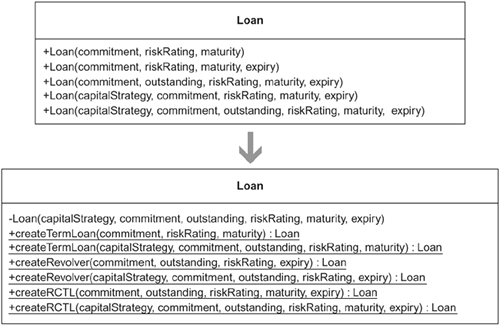
\includegraphics[width=0.8\textwidth]{figures/static-factory}
  \caption{static factory method}
  \label{fig:static-factory}
\end{figure}

\ascii{static factory method}具有很多优势,
\begin{enum}
  \eitem{\ascii{具有比构造函数更丰富的名称}}
  \eitem{\ascii{不必每次调用时都创建一个对象,有利于复用对象,提升性能}}
  \eitem{\ascii{返回类型可以是任何子类型的对象}}
\end{enum}

再以一个具体的实例来讲解\ascii{static factory method}的使用。按照美元的原始单位进行打印。注意:\ascii{dollar}的符号在前,而\ascii{cent}的符号在后。
\begin{enum}
  \eitem{\ascii{532 dollars => \$532}}
  \eitem{\ascii{1030 cents => 1030¢}}
\end{enum}

在面对这个问题时,抽象出了\ascii{DollarUnit}类,并提供两个\ascii{static factory method},以实现对\ascii{DollarUnit}实例生成的控制,并通过宏改善了\ascii{API}的可读性和方便性。

\begin{leftbar}
\begin{c++}
#ifndef INCL_DollarUnit_H_
#define INCL_DollarUnit_H_

#include "base/Keywords.h"
#include "money/Amount.h"
#include <ostream>

//////////////////////////////////////////////////////////////////////////
ABSTRACT(DollarUnit)
{
    static const DollarUnit& dollar();
    static const DollarUnit& cent();

    virtual void format(std::ostream& oss, const Amount& amount) const = 0;

protected:
    explicit DollarUnit(const Amount& convertionFactor);

private:
    const Amount convertionFactor;
};

//////////////////////////////////////////////////////////////////////////
#define DOLLAR DollarUnit::dollar()
#define CENT   DollarUnit::cent()

#endif
\end{c++}
\end{leftbar}

\begin{leftbar}
\begin{c++}
#include "money/DollarUnit.h"
#include "base/Keywords.h"
#include <string>

namespace
{
    struct Dollar : DollarUnit
    {
        Dollar(const Amount& convertionFactor)
         : DollarUnit(convertionFactor) {}

    private:
        OVERRIDE void format(std::ostream& oss, const Amount& amount) const
        {
            oss << "$" << amount;
        }
    };

    struct Cent : DollarUnit
    {
        Cent(const Amount& convertionFactor)
         : DollarUnit(convertionFactor) {}

    private:
        OVERRIDE void format(std::ostream& oss, const Amount& amount) const
        {
            oss << amount << "¢";
        }
    };
}

const Amount CENT_CONV_FACTOR   = 1;
const Amount DOLLAR_CONV_FACTOR = 100 * CENT_CONV_FACTOR;

const DollarUnit& DollarUnit::dollar()
{
    static Dollar dollar(DOLLAR_CONV_FACTOR);
    return dollar;
}

const DollarUnit& DollarUnit::cent()
{
    static Cent cent(CENT_CONV_FACTOR);
    return cent;
}

DollarUnit::DollarUnit(const Amount& convertionFactor)
 : convertionFactor(convertionFactor)
{
}
\end{c++}
\end{leftbar}

\begin{regulation}
通过私有构造函数强化不可实例化能力
\end{regulation}

以早期\ascii{boost}实现单态的技术为例讲解这个问题。

\begin{leftbar}
\begin{c++}
template<typename T>
struct Singleton
{
    static T& getInstance()
    {
        static T instance;
        return instance;
    }

private:
    Singleton& operator=(const Singleton&);
    Singleton(const Singleton&);

protected:
    Singleton() {}
};

#define SINGLETON(object) struct object : Singleton<object>
\end{c++}
\end{leftbar}

\begin{regulation}
避免创建不必要的对象
\end{regulation}

对象创建和销毁是有代价的,尤其在关乎性能的对象创建和销毁时,需要特别地关注。

这时出现了很多技术来解决这方面的问题,对象池技术和\ascii{Flyweight}模式是最常见的技术,例如线程池,数据库连接池,网络连接池等等。

参考实例可参见\ascii{Joshua Bloch}所著的\ascii{《Effective Java》},规则同样适用于\ascii{C++}。

\end{content}

\section{Inheritance, Polymorphism}

\begin{content}

\begin{regulation}
优先提供抽象的接口定义,并按接口编程
\end{regulation}

按接口编程是面向对象中最重要的原则之一。对业务抽象的接口往往表现为明确的契约关系,在\ascii{C++}语言中,虽然没有接口这样的概念,但已经存在成熟的设计方案。

\begin{leftbar}
\begin{c++}
namespace details
{
   template <typename T>
   struct Interface
   {
      virtual ~Interface() {}
   };
}

#define INTERFACE(type) struct type : ::details::Interface<type>
\end{c++}
\end{leftbar}

使用上述提供的\ascii{INTERFACE}宏,在定义一个接口时,可以省去对虚拟析构函数的重复实现。

\begin{leftbar}
\begin{c++}
INTERFACE(Runnable)
{
    virtual void run() = 0;
}
\end{c++}
\end{leftbar}

\begin{regulation}
避免从并非设计为基类的类中继承
\end{regulation}

\ascii{C++}并没有提供像\ascii{Java}语言一样的\ascii{final}关键字来组织类被继承的机制。通常情况下,所有的\ascii{C++}类都可以被继承。

但是有些类最初并不是以基类的角度进行设计的,这种类的往往却拥有\ascii{public non-virtual}析构函数,当子类的析构函数需要释放特定资源时,将发生未定义的行为。

如果你试图继承\ascii{string}或\ascii{STL}的其他容器,将走上这条不归路。

是否拥有何种技术提供类似\ascii{Java}语言一样的\ascii{final}关键字的机制呢,以便向读者透露出此类不可被继承的设计意图?其实\ascii{C++ 11}标准已经将\ascii{final}列为关键字,支持了这项语义。在此之前,也有类似的模拟技术实现\ascii{final}的功能,但实现复杂了一点,在此不进行详细阐述了。

但需要注意有的类虽然其析构函数是\ascii{public non-virtual}\footnote{此类为继承而生,但不具有多态性的类应该定义一个protected non-vritual destructor。},但天生是为继承而生的,它唯一特别的是不具有多态性,这样的类不属于此条例。虽然它具有\ascii{public non-virtual destructor},但它就是为继承而生的。例如,\ascii{std::input\_iterator\_tag, std::unary\_function}等标准库中的类。可惜的是,这条规则往往没有得到大家的认识,在面对这样的问题时,大家习惯了为这样的类定义个\ascii{public non-virtual destructor},请建议不要那么做了。

\begin{regulation}
考虑使用\ascii{virtual}函数声明非\ascii{public},而将\ascii{public}函数声明非\ascii{virtual}
\end{regulation}

此方法常被称为\ascii{NVI(non-virtual interface)},它是实现\ascii{Template Method Pattern}独特的一种表现形式。\ascii{Template Method}在父类中以一个\ascii{public}接口实现算法的骨架,并以\ascii{private virtual}挂接许多回调钩子供子类改写。

\begin{regulation}
区分\ascii{pure virtual, virtual, non-virtual}函数的语义
\end{regulation}

\ascii{pure virtual}是为了让子类只继承其接口;\ascii{virtual}是让子类继承接口和一份默认的实现;\ascii{non-virtual}是让子类继承其接口和一份强制性的实现。

当定义一个类时,清晰、准确的使用这三个特性,有助于别人理解类设计的意图。

\begin{regulation}
改写\ascii{virtual}函数时,提供显式的\ascii{override}标示
\end{regulation}

在子类中改写虚函数时,提供显式的\ascii{override}将改善其\ascii{API}的可读性,并增强了编译器的安全性检查。

\begin{leftbar}
\begin{c++}
#include "base/Keywords.h"
#include "base/Status.h"

INTERFACE(BbCfgListener)
{
    virtual Status onRbConfiging() = 0;     
    virtual void onRbCfgFailed() = 0;
};
\end{c++}
\end{leftbar}

\begin{leftbar}
\begin{c++}
#include "bb/role/BbCfgListener.h"

struct BbState : BbCfgListener
{
    BbState();    
   
    Status confirm();
    Status rollback();
    void   release();

private:
    Status onRbConfiging() override; 
    void   onRbCfgFailed() override;

private:    
    enum{ IDLE, ACTIVE, RECFG } state;
};
\end{c++}
\end{leftbar}

但可惜\ascii{override}关键字直到\ascii{C++ 11}才被列入标准,此时提供类似的机制是一件值得做的工作。

\begin{leftbar}
\begin{c++}
#define OVERRIDE virtual
\end{c++}
\end{leftbar}

只不过此处的\ascii{OVERRIDE}需要在函数头部进行声明,当然也缺乏了编译器的安全性检查。它的存在仅仅是为了改善\ascii{API}的意图。

\begin{leftbar}
\begin{c++}
#include "bb/role/BbCfgListener.h"

struct BbState : BbCfgListener
{
    BbState();    
   
    Status confirm();
    Status rollback();
    void   release();

private:
    OVERRIDE Status onRbConfiging(); 
    OVERRIDE void   onRbCfgFailed();

private:    
    enum{ IDLE, ACTIVE, RECFG } state;
};
\end{c++}
\end{leftbar}

\begin{regulation}
为多态基类声明为\ascii{virtual destructor}
\end{regulation}

何时需要给类增加\ascii{virtual destructor}常常让人抓狂。记住两点规则:

\begin{enum}
  \eitem{\ascii{As base class}}
  \eitem{\ascii{Polymorphic}}
\end{enum}

这两个条件必须同时满足,才为类增加\ascii{virtual destructor}。一般地,如果一个类包含虚函数时,就为它增加\ascii{virtual destructor}。

但需要注意的是,为继承而生,但没有多态的语义时,\ascii{Herb Sutter, Andrei Alexandrescu}建议显式地定义\ascii{protected non-vritual destructor}。可惜标准库并没有这么做,例如\ascii{std::input\_iterator\_tag, std::unary\_function}等标准库中的类。

但这不妨碍我们这样去设计,以便透露出本类只可继承,并无多态的设计意图。

\begin{regulation}
禁止在\ascii{constructor, destructor}中调用虚函数
\end{regulation}

在\ascii{constructor, destructor}期间,子类对象尚未构造,或已经销毁,所以在其父类的\ascii{constructor, destructor}中调用虚函数未能像我们期望的那样发生多态行为,所以禁止在\ascii{constructor, destructor}中调用虚函数。

\begin{regulation}
绝不重定义继承而来的\ascii{non-virtual}函数;也绝不重定义继承而来的缺省参数值
\end{regulation}

这是因为其重定义没有发生期望的多态行为,所以被建议不适用,以免产生反直觉的行为。

\begin{regulation}
避免遮掩继承而来的名称
\end{regulation}

这是\ascii{C++}在嵌套作用域的名字隐藏机制在类作用域中的一个具体表现形式。当出现这些特殊的异常的情况时,往往能嗅探出不良命名和设计的坏味道。

\begin{regulation}
使用函数对象表示策略
\end{regulation}

策略模式是一种最常见的设计模式之一,\ascii{C++}语言中,常常使用函数对象来实现。

例如\ascii{std::sort}中实现的排序,使用\ascii{Comparator}方便用户定制比较规则。

\begin{leftbar}
\begin{c++}
template<typename Iterator, typename Comparator>
void sort(Iterator first, Iterator last, Comparator comp);
\end{c++}
\end{leftbar}

\end{content}
